% \iffalse meta-comment
%<*internal>
\iffalse
%</internal>
%<*readme>
----------------------------------------------------------------
tikzmark --- remembering absolute positioning with TikZ
E-mail: stacey@math.ntnu.no
Released under the LaTeX Project Public License v1.3c or later
See http://www.latex-project.org/lppl.txt
----------------------------------------------------------------

The tikzmark package defines a command to "remember" a position
on a page for later (or earlier) use, primarily (but not
exclusively) with TikZ.
%</readme>
%<*internal>
\fi
\def\nameofplainTeX{plain}
\ifx\fmtname\nameofplainTeX\else
  \expandafter\begingroup
\fi
%</internal>
%<*install>
\input docstrip.tex
\keepsilent
\askforoverwritefalse
\preamble
----------------------------------------------------------------
tikzmark --- remembering absolute positioning with TikZ.
E-mail: stacey@math.ntnu.no
Released under the LaTeX Project Public License v1.3c or later
See http://www.latex-project.org/lppl.txt
----------------------------------------------------------------

\endpreamble
\postamble

Copyright (C) 2011 by Andrew Stacey <stacey@math.ntnu.no>

This work may be distributed and/or modified under the
conditions of the LaTeX Project Public License (LPPL), either
version 1.3c of this license or (at your option) any later
version.  The latest version of this license is in the file:

http://www.latex-project.org/lppl.txt

This work is "maintained" (as per LPPL maintenance status) by
Andrew Stacey.

This work consists of the file  tikzmark.dtx
and the derived files           tikzmark.ins,
                                tikzmark.pdf,
                                tikzlibrarytikzmark.code.tex, and
                                tikzmarklibrarylistings.code.tex

\endpostamble
\usedir{tex/latex/tikzmark}
\generate{
  \file{tikzlibrarytikzmark.code.tex}{\from{\jobname.dtx}{tikzlibrary}}
}
\generate{
  \file{tikzmarklibrarylistings.code.tex}{\from{\jobname.dtx}{listings}}
}
%</install>
%<install>\endbatchfile
%<*internal>
\usedir{source/latex/tikzmark}
\generate{
  \file{\jobname.ins}{\from{\jobname.dtx}{install}}
}
\nopreamble\nopostamble
\usedir{doc/latex/demopkg}
\generate{
  \file{README.txt}{\from{\jobname.dtx}{readme}}
}
\ifx\fmtname\nameofplainTeX
  \expandafter\endbatchfile
\else
  \expandafter\endgroup
\fi
%</internal>
%<*package>
\NeedsTeXFormat{LaTeX2e}
\ProvidesPackage{tikzmark}[2012/10/24 v1.0 TikZmark]
%</package>
%<*driver>
\documentclass{ltxdoc}
\usepackage[T1]{fontenc}
\usepackage{lmodern}
%\usepackage{morefloats}
\usepackage{tikz}
\usetikzlibrary{tikzmark}
\usepackage[numbered]{hypdoc}
\definecolor{lstbgcolor}{rgb}{0.9,0.9,0.9} 
 
\usepackage{listings}
\lstloadlanguages{[LaTeX]TeX}
\lstset{gobble=2,breakatwhitespace=true,breaklines=true,language=TeX}
 
\usepackage{fancyvrb}

\newenvironment{example}
  {\VerbatimEnvironment
   \begin{VerbatimOut}[gobble=2]{example.out}}
  {\end{VerbatimOut}
   \begin{center}
%   \setlength{\parindent}{0pt}
   \fbox{\begin{minipage}{.9\linewidth}
     \lstset{breakatwhitespace=true,breaklines=true,language=TeX,basicstyle=\small}
     \lstinputlisting[]{example.out}
   \end{minipage}}

   \fbox{\begin{minipage}{.9\linewidth}
     \input{example.out}
   \end{minipage}}
\end{center}
}
\EnableCrossrefs
\CodelineIndex
\RecordChanges
\begin{document}
  \DocInput{\jobname.dtx}
\end{document}
%</driver>
% \fi
%
%
% \CharacterTable
%  {Upper-case    \A\B\C\D\E\F\G\H\I\J\K\L\M\N\O\P\Q\R\S\T\U\V\W\X\Y\Z
%   Lower-case    \a\b\c\d\e\f\g\h\i\j\k\l\m\n\o\p\q\r\s\t\u\v\w\x\y\z
%   Digits        \0\1\2\3\4\5\6\7\8\9
%   Exclamation   \!     Double quote  \"     Hash (number) \#
%   Dollar        \$     Percent       \%     Ampersand     \&
%   Acute accent  \'     Left paren    \(     Right paren   \)
%   Asterisk      \*     Plus          \+     Comma         \,
%   Minus         \-     Point         \.     Solidus       \/
%   Colon         \:     Semicolon     \;     Less than     \<
%   Equals        \=     Greater than  \>     Question mark \?
%   Commercial at \@     Left bracket  \[     Backslash     \\
%   Right bracket \]     Circumflex    \^     Underscore    \_
%   Grave accent  \`     Left brace    \{     Vertical bar  \|
%   Right brace   \}     Tilde         \~}
%
%
% \changes{1.0}{2011/05/03}{Converted to DTX file}
%
% \DoNotIndex{\newcommand,\newenvironment}
%
% \providecommand*{\url}{\texttt}
% \GetFileInfo{tikzmark.dtx}
% \title{The \textsf{tikzmark} package}
% \author{Andrew Stacey \\ \url{stacey@math.ntnu.no}}
% \date{\fileversion~from \filedate}
%
%
% \maketitle
%
% 
% \section{Introduction}
%
% The \Verb+\tikzmark+ macro burst onto the scene in a blaze of glory on \href{http://tex.stackexchange.com}{TeX-SX}.
% Since then, it has proved embarrassingly (to its original author) popular.
% The idea behind it is extremely simple: that the machinery underneath TikZ provides a way to ``mark'' a point on a page for further use.
% This functionality is already provided by several other packages.
% The point of this one is that as TikZ can provide this feature, if already loading TikZ then it makes sense to use the TikZ version than another version.
% Moreover, if the goal is to use these marks with some TikZ code then this version is already set up for that purpose (not that it would be exactly difficult to add this to any of the other implementations).
%
% \section{Use}
%
% Using the \Verb+\tikzmark+ is extremely simple.
% You need to load the \Verb+tikz+ package and then load \Verb+tikzmark+ as a \Verb+tikzlibrary+.
% Thus in your preamble you should have something like:
%
% \begin{lstlisting}
% \usepackage{tikz}
% \usetikzlibrary{tikzmark}
% \end{lstlisting}
%
% In your document, you can now type \Verb+\tikzmark{<name>}+ at a point that you want to remember.
% This will save a mark with name \Verb+<name>+ for use later (or earlier).
% To use it in a \Verb+\tikz+ or \Verb+tikzpicture+, simply use the \Verb+pic+ coordinate system:
%
% \begin{lstlisting}
% \tikz[remember picture] \draw[overlay] (0,0) -- (pic cs:<name>);
% \end{lstlisting}
%
% There are two important points to note:
%
% \begin{enumerate}
% \item The enveloping \Verb+\tikz+ or \Verb+tikzpicture+ must have the key \Verb+remember picture+ set.
%
% This is because of how TikZ coordinates work.
% The coordinates inside a TikZ picture are relative to its origin, so that origin can move around on the page and not affect the internals of the picture.
% To use a point outside the picture, therefore, the current picture not only has to know where that point is on the page it also has to know where it is on the page.
% Hence the \Verb+remember picture+ key must be set.
% \item The drawing command must have the \Verb+overlay+ key set (or be in a scope or picture where it is set).
% 
% This is to keep the bounding box of the current picture under control.
% Otherwise, it would grow to encompass the remembered point as well as the current picture.
% \end{enumerate}
%
% 
%
% \section{History}
%
% I wrote the original \Verb+\tikzmark+ macro in 2009 for use in lecture slides prepared with the \Verb+beamer+ package.
% It's original definition was:
%
% \begin{lstlisting}
% \newcommand{\tikzmark}[1]{\tikz[overlay,remember picture] \node (#1) {};}
% \end{lstlisting}
%
% Its first use was thus the (inelegant) code:
%
% \begin{lstlisting}
% \begin{frame}
% \frametitle{Structure of Continuous Functions}
%
% \begin{tikzpicture}[overlay, remember picture]
% \useasboundingbox (0,0);
% \draw<2-|trans: 0|handout: 0>[red,->] (bsp) .. controls +(-1,-1) and ($(cnvs.north)+(1,1)$) .. ($(cnvs.north)+(0,1)$) .. controls ($(cnvs.north)+(-1,1)$) and +(-1,0) .. (cnvs.north);
% \draw<3-|trans: 0|handout: 0>[green!50!black,->] (cplt) .. controls +(-1,-1) and +(-1,0) .. (mcplt.north);
% \draw<4-|trans: 0|handout: 0>[blue,->] (norm) .. controls +(-1,-.5) and ($(nvs.north)+(0,1.5)$) .. ($(nvs.north)+(0,1.5)$) .. controls ($(nvs.north)+(-1.5,1.5)$) and +(-1.5,0) .. (nvs.north);
% \draw<5-|trans: 0|handout: 0>[purple,->] (vector) .. controls +(-1,-1) and ($(vsp.north)+(2,2)$) .. ($(vsp.north)+(0,2)$) .. controls ($(vsp.north)+(-2,2)$) and +(-2,0) .. (vsp.north);
% \end{tikzpicture}
%
% \begin{theorem}
% \centering
% \(\big(C([0,1],\R),d_\infty\big)\) \\
% is a \\
% \alert{Banach\tikzmark{bsp} space}
% \end{theorem}
%
% \pause
% \bigskip
%
% \begin{itemize}
% \item[\tikzmark{cnvs}] {\color<.(2)->{green!50!black}Comp\tikzmark{cplt}lete} {\color<.(3)->{blue}nor\tikzmark{norm}med} {\color<.(4)->{purple}vector\tikzmark{vector} space}.
%
% \bigskip
% \bigskip
% \pause
%
% \begin{itemize}[<+->]
% \item[\tikzmark{mcplt}] {\color{green!50!black}Cauchy sequences converge.}
% \medskip
% \item[\tikzmark{nvs}] {\color{blue}Metric from a norm.}
% \medskip
% \item[\tikzmark{vsp}] {\color{purple}Functions behave like vectors.}
% \end{itemize}
% \end{itemize}
%
% \end{frame}
% \end{lstlisting}
%
% This produced, on the final slide, Figure~\ref{fig:tikzmarkex}.
%
% \begin{figure}
% \centering
% 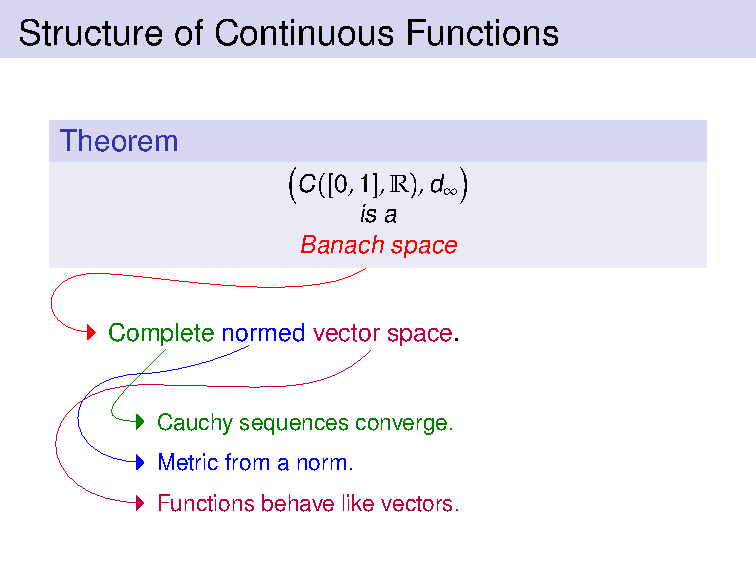
\includegraphics{tikzmark_example}
% \caption{First use of tikzmark}
% \label{fig:tikzmarkex}
% \end{figure}
%
% Its first appearance on \href{http://tex.stackexchange.com}{TeX-SX} was in an \href{http://tex.stackexchange.com/a/316/86}{answer} to a question about how to put overlapping braces on a mathematical text.
% This was in July 2010.
% The opening statement of the answer was not overly encouraging: ``This may not be the best solution\dots''.
% And for a macro that would go on to become quite ubiquitous, its initial appearance only garnered it 2 votes.
%
% However, it started out in life as a useful macro for me and as such I found more uses for it in my own code and thus more opportunity for using it to answer questions on TeX-SX.
% The one that seems to have been where it got noticed came in \href{http://tex.stackexchange.com/a/1570/86}{August 2010}, again about putting braces in text but in a more complicated fashion.
% From this answer, it got picked up, picked over, and picked apart.
% A common use was in highlighting or adding marks to text.
%
% Gradually, as it got used, it developed.
% A major revision dates from an answer given in \href{http://tex.stackexchange.com/a/50054/86}{March 2012} where the question was actually about \Verb+\tikzmark+.
% This version added two important features: a TikZ coordinate system for referencing saved marks directly and the ability to refer to marks earlier in the document than they are defined (the mechanism for remembering points uses the \Verb+aux+ file anyway so this was more about exposing the information earlier than anything complicated).
% Then in October 2012 there was a  \href{http://tex.stackexchange.com/q/79121/86}{question} where it would have been useful to remember which page the mark was on and a \href{http://tex.stackexchange.com/q/79762/86}{question} where for some reason using the \Verb+\tikz+ macro didn't work so the \Verb+\pgfmark+ macro was introduced.
%
% \section{Usage}
%
% This package defines the following commands and usable stuff.
%
% \begin{enumerate}
% \item \Verb+\tikzmark+\oarg{drawing command}\marg{name}
%
% The mandatory argument is the name of the mark to be used to refer back to this point later.
%
% The \Verb+\tikzmark+ command can take an optional parameter which is some drawing command that can be put in a \Verb+\tikz ... ;+ command.
% This drawing command can be used to place a node or something similar at the marked point, or to set some \Verb+\tikzset+ keys .
% Sometimes this can be useful.
% Note, though, that if this is used to define an offset coordinate then this will only be available in the document \emph{after} the \Verb+\tikzmark+ command, even on later runs.
%
% \item \Verb+\pgfmark+\marg{name}
%
% This is a more basic form of the \Verb+\tikzmark+ which doesn't use any of the \Verb+\tikz+ overhead.
% One advantage of this command is that it doesn't create an \Verb+hbox+.
% 
% \item \Verb+\iftikzmark+\marg{name}\marg{true code}\marg{false code}
%
% This is a simple conditional to test if a particular mark is available.
% It executes \Verb+true code+ if it is and \Verb+false code+ if not.
%
% \item \Verb+(pic cs:<name>)+ or \Verb+(pic cs:<name>,<coordinate>)+
%
% This is the method for referring to a position remembered by \Verb+\tikzmark+ as a coordinate in a \Verb+tikzpicture+ environment (or \Verb+\tikz+ command).
% If the extra \Verb+coordinate+ is specified then this is used in case the mark \Verb+name+ has not yet been defined (this can be useful for defining code that does something sensible on the first run).
%
% \item \Verb+/tikz/save picture id=<name>+
%
% This is the TikZ key that is used by \Verb+\tikzmark+ to actually save the connection between the name and the picture coordinate.
% It can be used on an arbitrary picture to save its origin.
%
% \item \Verb+/tikz/if picture id=#1#2#3+
%
% This is a key equivalent of the \Verb+\iftikzmark+ command.
%
% \item \Verb+/tikz/next page+, \Verb+/tikz/next page vector+
%
% It is possible to refer to a mark on a different page to the current page.
% When this is done, the mark is offset by a vector stored in the key \Verb+/tikz/next page vector+.
% The key \Verb+/tikz/next page+ can be used to set this to certain standard vectors by specifying where the ``next page'' is considered as lying corresponding to the current page.
% Possible values are (by default) \Verb+above+, \Verb+below+, \Verb+left+, \Verb+right+, and \Verb+ignore+.
% (The last one sets the vector to the zero vector.)
%
% \end{enumerate}
%
% \section{Examples and Extras}
%
% The \Verb+\tikzmark+ command has been used in numerous answers on \href{http://tex.stackexchange.com}{TeX-SX}.
% The following is a random selection.
%
% \begin{enumerate}
% \item 
% \end{enumerate}
%
% Some of these have been gathered into extra libraries that are loaded via \Verb+\usetikzmarklibrary+.
% 
%
% \section{Acknowledgements}
%
% The \Verb+\tikzmark+ macro has been used and abused by many users of \href{http://tex.stackexchange.com}{TeX-SX}.
% Of particular note (but in no particular order) are \href{}{Peter Grill}, \href{}{Gonzalo Medina}, and \href{}{Claudio Fiandrino}.
% 
%
% \StopEventually{}
%
% \section{Implementation}
%
% \iffalse
%<*tikzlibrary>
% \fi
%
%    \begin{macrocode}
\tikzset{%
  remember picture with id/.style={%
    remember picture,
    overlay,
    save picture id=#1,
  },
%    \end{macrocode}
% Not totally happy with using \Verb+every picture+ here as it's too easily overwritten by the user.
% Maybe it would be better to patch \Verb+endtikzpicture+ directly.
%    \begin{macrocode}
  every picture/.append style={%
    execute at end picture={%
      \ifpgfrememberpicturepositiononpage%
      \edef\pgf@temp{%
        \noexpand\write\noexpand\pgfutil@auxout{%
        \string\savepicturepage{\pgfpictureid}{\noexpand\thepage}}}%
      \pgf@temp
      \fi%
    },
  },
%    \end{macrocode}
% The positions are already recorded in the \Verb+aux+ file, all we really need to do is provide them with better names.
%    \begin{macrocode}
  save picture id/.code={%
      \immediate\write\pgfutil@auxout{%
        \string\savepointas{#1}{\pgfpictureid}}%
  },
%    \end{macrocode}
% Provides a way to test if a picture has already been saved (in particular, can avoid errors on first runs)
%    \begin{macrocode}
  if picture id/.code args={#1#2#3}{%
    \@ifundefined{save@pt@#1}{%
      \pgfkeysalso{#3}%
    }{
      \pgfkeysalso{#2}%
    }
  },
%    \end{macrocode}
% Page handling
%    \begin{macrocode}
  next page/.is choice,
  next page vector/.initial={\pgfqpoint{0pt}{0pt}},
  next page/below/.style={%
    next page vector={\pgfqpoint{0pt}{-\the\paperheight}}%
  },
  next page/above/.style={%
    next page vector={\pgfqpoint{0pt}{\the\paperheight}}%
  },
  next page/left/.style={%
    next page vector={\pgfqpoint{-\the\paperwidth}{0pt}}%
  },
  next page/right/.style={%
    next page vector={\pgfqpoint{\the\paperwidth}{0pt}}%
  },
  next page/ignore/.style={%
    next page vector={\pgfqpoint{0pt}{0pt}}%
  },
}
%    \end{macrocode}
%
% \begin{macro}{\savepointas}
% This is what gets written to the \Verb+aux+ file.
%    \begin{macrocode}
\def\savepointas#1#2{%
  \expandafter\gdef\csname save@pt@#1\endcsname{#2}%
}
\def\savepicturepage#1#2{%
  \expandafter\gdef\csname save@pg@#1\endcsname{#2}%
}
%    \end{macrocode}
% \end{macro}
%
% \begin{macro}{\tmk@labeldef}
% Auxiliary command for the coordinate system.
%    \begin{macrocode}
\def\tmk@labeldef#1,#2\@nil{%
  \def\tmk@label{#1}%
  \def\tmk@def{#2}%
}
%    \end{macrocode}
% \end{macro}
%
% \begin{macro}{pic}
% This defines the new coordinate system.
%    \begin{macrocode}
\tikzdeclarecoordinatesystem{pic}{%
  \pgfutil@in@,{#1}%
  \ifpgfutil@in@%
    \tmk@labeldef#1\@nil
  \else
    \tmk@labeldef#1,(0pt,0pt)\@nil
  \fi
  \@ifundefined{save@pt@\tmk@label}{%
    \tikz@scan@one@point\pgfutil@firstofone\tmk@def
  }{%
      \pgfsys@getposition{\csname save@pt@\tmk@label\endcsname}\save@orig@pic%
      \pgfsys@getposition{\pgfpictureid}\save@this@pic%
      \pgf@process{\pgfpointorigin\save@this@pic}%
      \pgf@xa=\pgf@x
      \pgf@ya=\pgf@y
      \pgf@process{\pgfpointorigin\save@orig@pic}%
      \advance\pgf@x by -\pgf@xa
      \advance\pgf@y by -\pgf@ya
      \pgf@xa=\pgf@x
      \pgf@ya=\pgf@y
      \@ifundefined{save@pg@\csname save@pt@\tmk@label\endcsname}{}{%
        \@ifundefined{save@pg@\pgfpictureid}{}{%
          \pgfkeysvalueof{/tikz/next page vector}%
          \advance \pgf@xa by \csname save@pg@\csname save@pt@\tmk@label\endcsname\endcsname\pgf@x\relax
\advance \pgf@ya by \csname save@pg@\csname save@pt@\tmk@label\endcsname\endcsname\pgf@y\relax
          \advance \pgf@xa by -\csname save@pg@\pgfpictureid\endcsname\pgf@x\relax
\advance \pgf@ya by -\csname save@pg@\pgfpictureid\endcsname\pgf@y\relax
        }%
      }%
      \pgf@x=\pgf@xa
      \pgf@y=\pgf@ya
    }%
  }
%    \end{macrocode}
% \end{macro}
%
% \begin{macro}{\tikzmark}
%    \begin{macrocode}
\newcommand\tikzmark[2][]{%
\tikz[remember picture with id=#2] #1;}
%    \end{macrocode}
% \end{macro}
%
% \begin{macro}{\pgfmark}
%    \begin{macrocode}
\newcommand\pgfmark[1]{%
    \global\advance\pgf@picture@serial@count by1\relax%
    \edef\pgfpictureid{pgfid\the\pgf@picture@serial@count}%
%    \hbox to0pt{%
      \pgfsys@markposition{\pgfpictureid}
%    }%
    \edef\pgf@temp{%
      \noexpand\write\noexpand\pgfutil@auxout{%
        \string\savepicturepage{\pgfpictureid}{\noexpand\thepage}}}%
    \pgf@temp
    \immediate\write\pgfutil@auxout{%
      \string\savepointas{#1}{\pgfpictureid}}%
  }
%    \end{macrocode}
% \end{macro}
%
% \begin{macro}{\iftikzmark}
%    \begin{macrocode}
\newcommand\iftikzmark[3]{%
    \@ifundefined{save@pt@#1}{%
      #3%
    }{%
      #2%
    }%
  }%
%    \end{macrocode}
% \end{macro}
%
% \begin{macro}{\usetikzmarkextra}
%    \begin{macrocode}
\def\usetikzmarkextra{\pgfutil@ifnextchar[{\use@tikzmarklibrary}{\use@@tikzmarklibrary}}%}
\def\use@tikzmarklibrary[#1]{\use@@tikzmarklibrary{#1}}
\def\use@@tikzmarklibrary#1{%
  \edef\pgf@list{#1}%
  \pgfutil@for\pgf@temp:=\pgf@list\do{%
    \expandafter\pgfkeys@spdef\expandafter\pgf@temp\expandafter{\pgf@temp}%
    \ifx\pgf@temp\pgfutil@empty
    \else
      \expandafter\ifx\csname tikzmark@library@\pgf@temp @loaded\endcsname\relax%
      \expandafter\global\expandafter\let\csname tikzmark@library@\pgf@temp @loaded\endcsname=\pgfutil@empty%
      \expandafter\edef\csname tikzmark@library@#1@atcode\endcsname{\the\catcode`\@}
      \expandafter\edef\csname tikzmark@library@#1@barcode\endcsname{\the\catcode`\|}
      \catcode`\@=11
      \catcode`\|=12
      \pgfutil@InputIfFileExists{tikzmarklibrary\pgf@temp.code.tex}{}{
          \PackageError{tikzmark}{I did not find the tikzmark extras library '\pgf@temp'.}{}
        }%
      \catcode`\@=\csname tikzmark@library@#1@atcode\endcsname
      \catcode`\|=\csname tikzmark@library@#1@barcode\endcsname
      \fi%
    \fi
  }%
}

%    \end{macrocode}
% \end{macro}
%
% \iffalse
%</tikzlibrary>
% \fi
%
% \iffalse
%<*listings>
% \fi
%
% From \url{http://tex.stackexchange.com/q/79762/86}
%
%    \begin{macrocode}
\@ifpackageloaded{listings}{%
%    \end{macrocode}
%
% \begin{macro}{\iflst@linemark}
% A conditional to help with placing the mark at the first non-whitespace character.
%    \begin{macrocode}
    \newif\iflst@linemark
%    \end{macrocode}
% \end{macro}
%
% \begin{macro}{EveryLine}
% This hook places the mark at the start of the line.
%    \begin{macrocode}
\lst@AddToHook{EveryLine}{%
  \begingroup
  \advance\c@lstnumber by 1\relax
  \pgfmark{line-\lst@name-\the\c@lstnumber-start}%
  \endgroup
}
%    \end{macrocode}
% \end{macro}
%
% \begin{macro}{EOL}
% This hook places the mark at the end of the line and resets the conditional for placing the first mark.
%    \begin{macrocode}
\lst@AddToHook{EOL}{\pgfmark{line-\lst@name-\the\c@lstnumber-end}%
\global\lst@linemarktrue
}
%    \end{macrocode}
% \end{macro}
%
% \begin{macro}{OutputBox}
% Experimenting shows that this is the right place to set the mark at the first non-whitespace character.
% But we only want to do this once per line.
%    \begin{macrocode}
\lst@AddToHook{OutputBox}{%
  \iflst@linemark
  \pgfmark{line-\lst@name-\the\c@lstnumber-first}%
  \global\lst@linemarkfalse
  \fi
}
%    \end{macrocode}
% \end{macro}
%
% \begin{macro}{\tikzmk@lst@fnum}
% An auxiliary macro to figure out if the \Verb+firstnumber+ key was set.
% If so, it has the form \Verb+<number>\relax+.
% If not, it expands to a single token.
%    \begin{macrocode}
\def\tkzmk@lst@fnum#1\relax#2\@STOP{%
  \def\@test{#2}%
  \ifx\@test\@empty
  \def\tkzmk@lst@start{0}%
  \else
  \@tempcnta=#1\relax
  \advance\@tempcnta by -1\relax
  \def\tkzmk@lst@start{\the\@tempcnta}%
  \fi
}
%    \end{macrocode}
% \end{macro}
%
% \begin{macro}{Init}
% Adds a mark at the start of the listings environment.
%    \begin{macrocode}
\lst@AddToHook{Init}{%
  \expandafter\tkzmk@lst@fnum\lst@firstnumber\relax\@STOP
  \pgfmark{line-\lst@name-\tkzmk@lst@start-start}%
}
%    \end{macrocode}
% \end{macro}
%
% \begin{macrocode}
}{%
    \PackageError{tikzmark listings}{The listings package has not been loaded.}{}
}
%    \end{macrocode}
% \iffalse
%</listings>
% \fi
%
% \Finale

\endinput
